\documentclass[a4paper,16pt]{article}
%packages
\usepackage[margin=0.53in]{geometry}
\usepackage{sectsty}
\usepackage{graphicx}
\usepackage{listings}
\usepackage{subcaption}
\usepackage{setspace}
\usepackage{fancyhdr}
\usepackage{lastpage}
\usepackage{pxfonts}
%caption setup and page style
\captionsetup{font=large,labelfont=large}
\fancyfoot{} % clear all footer fields
\pagestyle{fancy}
\captionsetup{font=large,labelfont=large}
\usepackage{tocloft}
\sectionfont{\Huge\bfseries}
\subsectionfont{\Large \bfseries}
\renewcommand\cftsecpagefont{\LARGE}
\renewcommand\cftsubsecpagefont{\Large}

\fancyfoot[LE,RO]{\thepage} % page number in "outer" position of footer line
\fancyfoot[RE,LO]{} % other info in "inner" position of footer line
\rfoot{Page \thepage \hspace{1pt} of \pageref{LastPage}}
\setlength\cftbeforesubsecskip{20pt}
\setlength\cftaftertoctitleskip{20pt}
%language definitions and customizations
\lstset{
language={HTML},
keywords={input,html,body,head,form,span,select,option,br,h1,h2,div,textarea,id,class,name,label,script,link,rel,type,src,href,value,cols,rows},
keywordstyle=\bfseries,
numbers=left,frame=shadowbox,basicstyle=\ttfamily\large,
}
\lstset{
	language={Java},
	tabsize=2,
	keywords={String,char,boolean,Thread,public, void,setBackground,setForeground,drawString,setFont,class, Applet,extends,import,Font,drawLine,fillRect,drawOval,setColor,fillOval,drawArc,fillArc,applet,java,awt,new,start,stop,sleep,getTime,getInstance,format,repaint,catch,util,text,SimpleDateFormat,Button,TextField,setBounds,addActionListener,this,setLayout,setText,implements,ActionListener,event,add,getAudioclip,getSource,getCodeBase,play,audioClip,Image,getImage,getDocumentBase,drawImage,toString,readLine,StringBuffer,append,printStackTrace,openStream,TextArea,getParameter,setEditable,io,net},
	numbers=left,frame=shadowbox,basicstyle=\ttfamily\large,
}
\lstdefinelanguage{CSS}{
	keywords={color,background-image,margin,left,padding,font,weight,display,position,top,left,right,bottom,list,style,border,size,white,space,min,width, transition:, transform:, transition-property, transition-duration, transition-timing-function,height,line,height,text,align,margin-right,background,box,sizing,webkit,radius,cursor,float,transform},
	keywordstyle=\bfseries,
	showstringspaces=false,
}
\lstdefinelanguage{JavaScript}{
	keywords={typeof, new, true, false, catch, function, return, null, catch, switch, var, if, in, while, do, else, case, break,document,getElementById,innerHTML,value,write,window,location,reload,test,length}
	keywordstyle=\bfseries,
	morecomment=[s]{/*}{*/},
	morecomment=[l]//,
	morestring=[b]",
	morestring=[b]'
}
%beggining of the document
\begin{document}
	{
		\pagenumbering{arabic}
		{
			\renewcommand\contentsname{\Huge Contents}
			\renewcommand\cftsecfont{\LARGE}
			\renewcommand\cftsubsecfont{\Large}
			\doublespacing
			\doublespacing
			\doublespacing
			\tableofcontents
			\singlespacing
			\addtocontents{toc}{~\hfill\textbf{\Large Page}\par}
		}
	}
	\newpage
	\section{Assignment-1}
	\subsection{HTML form}
	\vspace{0.2in}
	\lstinputlisting[language=HTML]{code/form.html}
	\subsection{JavaScript}
	\lstinputlisting[language=JavaScript]{code/form.js}
	\subsection{CSS}
	\lstinputlisting[language=CSS]{code/style.css}
	\begin{figure}[h!]
		\includegraphics*[scale=0.25,width=1\linewidth]{code/form.png}
		\caption{\large form.html}
	\end{figure}
	\clearpage
	\section{Assignment-2}
	\subsection{Banner using applet}
	\lstinputlisting{code/Banner/Banner.java}
	\begin{figure}[h!]
		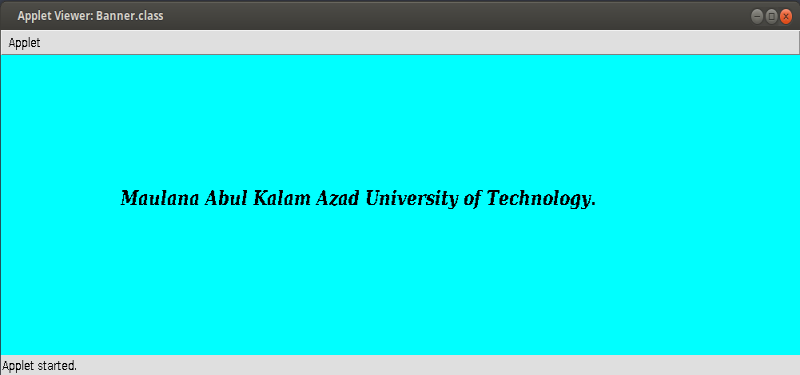
\includegraphics[scale=0.6,width=\linewidth]{code/Banner/Banner.png}
		\caption{Banner}
	\end{figure}
	\newpage
	\subsection{Generating shapes using applet}
	\lstinputlisting{code/shapes/GraphicsDemo.java}
	\begin{figure}[h!]
		\centering
		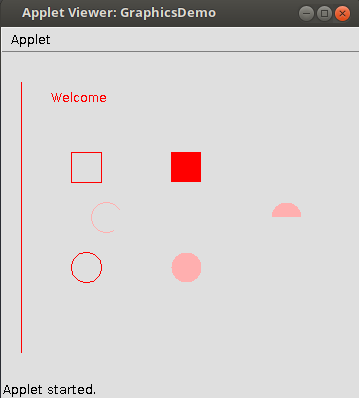
\includegraphics[scale=0.4,width=0.7\linewidth]{code/shapes/shapes.png}
		\caption{Different shapes}
	\end{figure}
	\newpage
	\subsection{Clock using applet}
	\lstinputlisting{code/Clock/DigiClock.java}
	\begin{figure}[h!]
		\centering
		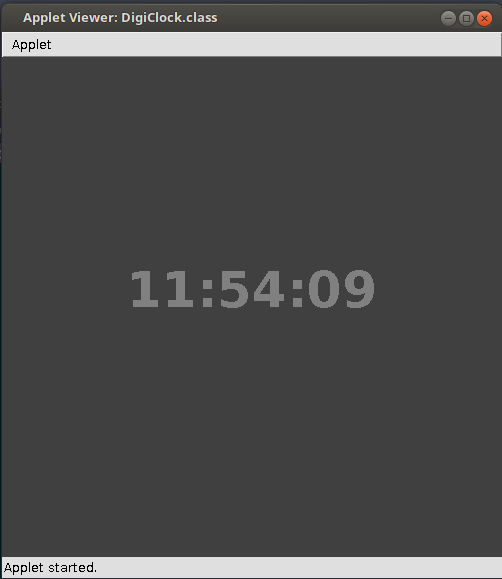
\includegraphics[width=8cm,height=6.5cm]{code/Clock/clock.png}
		\caption{Clock applet}
	\end{figure}
	\newpage
	\subsection{Event listener using Applet}
	\lstinputlisting{code/Listener/Listen.java}
	\begin{figure}[h!]
		\centering
		\begin{subfigure}[h]{0.36\linewidth}
			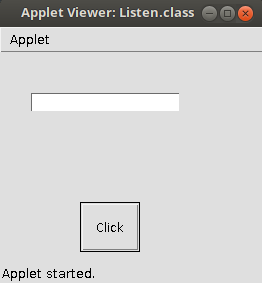
\includegraphics[width=\linewidth]{code/Listener/nclick}
			\caption{Before click}
		\end{subfigure}
		\hfill
		\begin{subfigure}[h]{0.39\linewidth}
			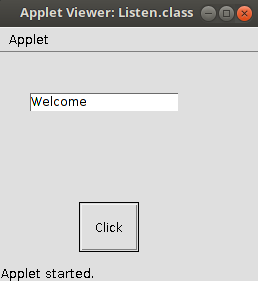
\includegraphics[width=\linewidth,height=1\linewidth]{code/Listener/click}
			\caption{After click}
		\end{subfigure}%
		\caption{A click event listener}
	\end{figure}
	\newpage
	\subsection{Playing sound using applet}
	\lstinputlisting{code/Sound/Sound.java}
	\newpage
	\subsection{Image Display using applet}
	\lstinputlisting{code/ImageDisplay/Imager.java}
	\begin{figure}[h]
		\centering
		
\includegraphics[width=0.5\linewidth]{code/ImageDisplay/image.png}
		\caption{Image Displayed using applet}
	\end{figure}
	\newpage
	\subsection{Reading a file using applet}
	\lstinputlisting{code/Files/Filer.java}
	\begin{figure}[h]
		\centering 
		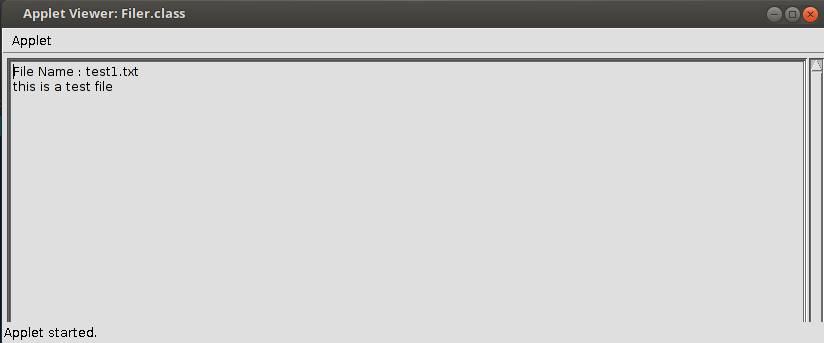
\includegraphics[scale=0.51]{code/Files/file.png}
		\caption{Reading a file using applet}
	\end{figure}
	
\end{document}